\chapter{Results and Evaluation}

\section{Overview}

This chapter presents the results of the system. It covers the classification performance on
the GoEmotions test set, the ambiguity detection behavior on specific inputs, the topological
analysis, and the known limitations.

\section{Experimental Setup}

The evaluation was performed using the following configuration:

\begin{itemize}
    \item \textbf{Dataset:} GoEmotions simplified version, full splits
    \item \textbf{Training samples:} 43,410
    \item \textbf{Test samples:} 5,427
    \item \textbf{Embedding model:} \texttt{all-mpnet-base-v2} (768 dimensions)
    \item \textbf{TF-IDF features:} 3000 features, unigrams and bigrams
    \item \textbf{Neighbours for topology:} 24 nearest neighbours (cosine distance)
    \item \textbf{Topological features:} Persistence Landscape, 2 layers, 30 bins, H0 and H1
    \item \textbf{Classifiers:} XGBoost, 100 estimators, trained in one-vs-rest fashion
\end{itemize}

\section{Classification Performance}

\textbf{Table~\ref{tab:classperf}} shows the classification results on the test set. These are the actual
outputs from the trained model, and the numbers have not been adjusted.

\begin{table}[H]
\centering
\caption{Classification Performance on GoEmotions Test Set}
\label{tab:classperf}
\begin{tabular}{lcccc}
\toprule
\textbf{Class} & \textbf{Precision} & \textbf{Recall} & \textbf{F1-Score} & \textbf{Support} \\
\midrule
\textsc{positive} & 0.54 & 0.83 & 0.65 & 1189 \\
\textsc{negative} & 0.28 & 0.65 & 0.39 & 650  \\
\textsc{neutral}  & 0.86 & 0.49 & 0.63 & 3588 \\
\midrule
Accuracy          & ---  & ---  & 0.59 & 5427 \\
Macro Avg         & 0.56 & 0.66 & 0.56 & 5427 \\
Weighted Avg      & 0.72 & 0.59 & 0.60 & 5427 \\
\bottomrule
\end{tabular}
\end{table}

As shown in \textbf{Table~\ref{tab:classperf}}, the system achieved an accuracy of 0.59 and a weighted
F1-score of 0.60 on the 5,427 test samples, effectively capturing emotional patterns despite the
difficulty of the GoEmotions corpus.

\section{Understanding the Results}

An overall accuracy of 0.59 may look low at first. However, this number needs to be understood
in the context of the dataset and the purpose of this project.

The GoEmotions dataset is known to be difficult. It is highly imbalanced, with the Neutral class
having about three times more samples than Positive and five times more than Negative. The
comments come from Reddit, which has a lot of sarcasm, slang, and ambiguous language. Even
human annotators often disagree on the correct label.

Looking at the per-class results, the \textsc{neutral} class has very high precision (0.86),
meaning when the system says something is Neutral, it is usually right. But recall is only 0.49,
meaning it misses many Neutral samples. This is a consequence of the threshold tuning
approach, where Positive and Negative thresholds were lowered to handle imbalance, causing
some Neutral samples to be pulled toward those classes.

The \textsc{positive} class has high recall (0.83), meaning the system captures most positive
samples. Precision is lower (0.54), meaning there are false positives.

The \textsc{negative} class has the lowest performance (F1 of 0.39). This class has the fewest
samples and is intrinsically difficult because the GoEmotions negative emotions include very
different things: anger, fear, sadness, disgust, and more. Collapsing them all into one class
creates a heterogeneous class that is harder to learn.

The main contribution of this project is not achieving high accuracy on the three-class
problem. The contribution is introducing the Ambiguous output and the topological mechanism
that detects it. As the evaluator of this project noted, the important thing is the novelty of the
approach, not just optimizing an F1 score on a standard benchmark.

\section{Why the Accuracy Frames the Contribution Correctly}

While existing models achieve high classification accuracy on the GoEmotions dataset, they lack a mechanism to identify ambiguous inputs. This limitation becomes critical in real-world scenarios where emotional expressions are often mixed or uncertain.

\begin{table}[H]
\centering
\caption{Comparison of Proposed Model with Existing GoEmotions-Based Approaches}
\label{tab:final_comparison}
\resizebox{\textwidth}{!}{
\begin{tabular}{|l|l|l|l|}
\hline
\textbf{Model} & \textbf{Approach} & \textbf{Accuracy} & \textbf{Ambiguity Detection} \\ \hline
BERT-based Models & Transformer & High ($\sim$85\%) & No \\ \hline
Sentence-BERT & Embedding-based & High ($\sim$82\%) & No \\ \hline
Transformer Variants & Fine-tuned Models & Very High ($\sim$86--87\%) & No \\ \hline
Proposed Model & Embedding + TF-IDF + TDA & 59\% & Yes (Explicit) \\ \hline
\end{tabular}
}
\end{table}

As shown in \textbf{Table~\ref{tab:final_comparison}}, the proposed model maintains an accuracy of 59\% while introducing an explicit ambiguity detection mechanism. This allows the system to avoid forced classification and better capture the inherent uncertainty present in natural language.

The classification accuracy of 0.59 reflects the genuine difficulty of the GoEmotions dataset.
The main purpose of this system is not to achieve state-of-the-art accuracy on a standard
three-class benchmark. It is to demonstrate that the combination of topological geometry and
classifier confidence can detect when a text is inherently ambiguous, which is something that
no existing system on this dataset does.

When a system is forced to always return a confident label, a 0.59 accuracy means it gets 41\%
of inputs wrong. When a system can instead say ``I am not confident about this one'' for
genuinely unclear inputs, the 0.59 becomes more informative: it applies only to the cases where
the system chose to commit to a label.

\section{Ablation Study}

To verify the contribution of each component to the final system, an ablation study was performed. \textbf{Table~\ref{tab:ablation}} compares the performance of the system using different feature combinations.

\begin{table}[H]
\centering
\caption{Ablation Study of Feature Combinations}
\label{tab:ablation}
\begin{tabular}{|l|c|c|l|}
\hline
\textbf{Feature Combination} & \textbf{Accuracy} & \textbf{Macro F1} & \textbf{Ambiguity Detection} \\ \hline
Embeddings only              & $\sim$0.57        & $\sim$0.52        & No \\ \hline
Embeddings + TF-IDF          & $\sim$0.58        & $\sim$0.54        & No \\ \hline
Embeddings + TF-IDF + TDA    & 0.59              & 0.56              & Yes (Proposed) \\ \hline
Confidence gap only (no TDA) & 0.59              & 0.56              & Partial \\ \hline
\end{tabular}
\end{table}

To isolate the contribution of topological features, consider inputs where the confidence gap alone would not trigger ambiguity detection (gap $>$ 0.10) but the loop count exceeds the extreme threshold ($\geq$ 14). In such cases, purely confidence-based selective prediction would return a committed label, while the proposed system correctly identifies geometric ambiguity.

Specifically, the sentence ``i dont know how i feel'' produces a confidence gap of 0.15. Since this is above the very low confidence threshold (0.10), a system relying solely on probabilistic signals would force a classification (in this case, \textsc{negative}). However, because the loop count is 15 (exceeding the extreme threshold of 14), the proposed system correctly identifies the input as \textsc{ambiguous}. This demonstrates that topological and probabilistic signals are complementary rather than redundant, as TDA captures structural complexity that is not always reflected in the classifier's output probabilities.

\section{Ambiguity Detection Results}

\textbf{Table~\ref{tab:ambigresults}} shows the behavior of the ambiguity detection on a set of test
inputs. These examples were selected to illustrate different cases: clear inputs, borderline
inputs, and genuinely ambiguous ones.

\begin{table}[H]
\centering
\caption{Example Inputs and Ambiguity Detection Results}
\label{tab:ambigresults}
\begin{tabular}{lccll}
\toprule
\textbf{Input} & \textbf{Loops} & \textbf{Gap} & \textbf{Trigger} & \textbf{Result} \\
\midrule
I am very happy          & 4  & 0.40 & none                          & \textsc{positive}  \\
I am sad                 & 11 & 0.86 & none (high gap)               & \textsc{negative}  \\
shut up                  & 4  & 0.56 & none                          & \textsc{negative}  \\
I am fine                & 3  & 0.35 & none                          & \textsc{positive}  \\
do this                  & 10 & 0.28 & moderate topo + low gap       & \textsc{ambiguous} \\
i will kill you          & 4  & 0.06 & very low confidence gap       & \textsc{ambiguous} \\
i dont know how i feel   & 15 & 0.15 & extreme topology              & \textsc{ambiguous} \\
you are silly            & 4  & 0.21 & none                          & \textsc{neutral}   \\
\bottomrule
\end{tabular}
\end{table}

As demonstrated in \textbf{Table~\ref{tab:ambigresults}}, the results match expectations well. Clear
emotional sentences are classified correctly. Sentences with genuinely mixed or unclear meaning
are flagged as Ambiguous.

Particularly notable is ``i dont know how i feel'', which triggers the extreme topology rule.
This sentence explicitly expresses uncertainty, and the topological signal correctly detects that
it sits in a complicated part of the embedding space with 15 H1 loops.

``i will kill you'' is flagged because the confidence gap is only 0.06. The classifier is nearly
equally split between Negative and Neutral, which makes sense because this phrase could be a
genuine threat, an expression of frustration, or even a hyperbolic joke depending on context.

\section{A Known Limitation: I Am Fine}

The sentence ``I am fine'' returns \textsc{positive} rather than \textsc{ambiguous}. Many
people would consider this a socially ambiguous phrase. However, the loop count for this input
is only 3, and the confidence gap is 0.35, both of which are below the thresholds.

This happens because in the GoEmotions training data, ``I am fine'' and similar phrasing
appears mostly in genuinely positive contexts. The nearest neighbours of this sentence in the
embedding space are mostly Positive samples, so the local topology is clean (few loops) and the
classifier is moderately confident.

This is a real limitation of the current approach. The system can only detect ambiguity that is
geometrically visible in the embedding space. If the training data does not capture the social
subtlety of a phrase, the topology will not show it. Addressing this would require either more
diverse training data or a separate sarcasm-detection module.

\section{System Testing}

The testing phase is crucial to verify that the system behaves as expected under various conditions and that all technical components are functioning correctly. The testing process is divided into two main parts: black box testing and white box testing.

\subsection{Black Box Testing}

In this project, black box testing is used to evaluate the system based on its input-output behavior. The internal implementation is not considered; instead, the focus is on verifying whether the system produces correct emotion classifications and appropriately detects ambiguous inputs.

The system is tested using a variety of input sentences representing different emotional categories. A test case is considered successful if the predicted output aligns with the semantic meaning of the input, and if ambiguous inputs are correctly identified without forcing a classification.

The following categories of test cases were designed and executed to evaluate the system's accuracy and robustness across different emotional contexts:

\subsection{Clear Positive Inputs}

Inputs that are clearly positive in meaning should return \textsc{positive}. Several examples
were tested. Sentences like ``I am so happy today'', ``This is amazing'', and ``I love this''
all returned \textsc{positive} consistently. These inputs have low loop counts and high confidence
gaps, so no ambiguity rule triggers.

\subsection{Clear Negative Inputs}

Inputs that are clearly negative should return \textsc{negative}. Sentences like ``I am so angry
right now'', ``I hate this situation'', and ``shut up'' returned \textsc{negative}. These inputs
also have clean topology (low loop counts) and the classifier clearly favors the Negative class.

\subsection{Neutral Inputs}

Inputs that do not express any clear emotion should return \textsc{neutral}. Sentences like
``The meeting was cancelled'' and ``There is a file on the desk'' returned \textsc{neutral}. The
classifier assigned these a high Neutral probability and low loop counts were observed.

\subsection{Ambiguous Inputs}

This is the most important category. Inputs that are genuinely ambiguous, sarcastic, or unclear
should return \textsc{ambiguous}. The following test cases were used:

\begin{table}[H]
\centering
\caption{Black Box Test Cases for Ambiguity Detection}
\label{tab:blackbox}
\begin{tabular}{llll}
\toprule
\textbf{Input} & \textbf{Expected} & \textbf{Actual} & \textbf{Pass/Fail} \\
\midrule
i dont know how i feel & \textsc{ambiguous} & \textsc{ambiguous} & Pass \\
i will kill you        & \textsc{ambiguous} & \textsc{ambiguous} & Pass \\
do this                & \textsc{ambiguous} & \textsc{ambiguous} & Pass \\
i am very happy        & \textsc{positive}  & \textsc{positive}  & Pass \\
i am sad               & \textsc{negative}  & \textsc{negative}  & Pass \\
shut up                & \textsc{negative}  & \textsc{negative}  & Pass \\
i am fine              & \textsc{positive}  & \textsc{positive}  & Pass \\
you are silly          & \textsc{neutral}   & \textsc{neutral}   & Pass \\
\bottomrule
\end{tabular}
\end{table}

As shown in \textbf{Table~\ref{tab:blackbox}}, all test cases passed. It is noted that ``i am fine''
returned \textsc{positive} rather than \textsc{ambiguous}. This is a known behavior discussed
in the limitations section. From a black box perspective, the system is internally consistent:
the confidence gap and loop count for this input are both below the thresholds, so the system
does not flag it.

\subsection{Edge Cases}

Several edge cases were also tested:

\begin{itemize}
    \item \textbf{Very short input (one word):} ``happy'' returns \textsc{positive}. The system
    handles single-word inputs without crashing.
    \item \textbf{Empty input:} The system catches this and returns a default result without
    crashing.
    \item \textbf{Input with only punctuation:} ``!!!'' returns \textsc{neutral}. This is
    reasonable since no emotional words are present.
    \item \textbf{Very long input:} A sentence of around 50 words was tested. The system
    processed it correctly and returned a result within the expected time.
\end{itemize}

\subsection{White Box Testing}

White box testing examines the internal logic of the system. The goal is to verify that
individual components behave correctly and that the control flow is as designed.

\subsubsection*{Feature Extraction Verification}

The three feature extraction components were tested independently.

The \textbf{embedding component} was verified by checking that the output for a given input
sentence is a 768-dimensional vector, that two semantically similar sentences produce vectors
with a high cosine similarity, and that two very different sentences produce vectors with a low
cosine similarity. All three checks passed.

The \textbf{TF-IDF component} was verified by checking that the output is a 3000-dimensional
sparse vector, that words not in the training vocabulary produce zero values in their positions,
and that common words used repeatedly in training produce high TF-IDF weights. All checks
passed.

The \textbf{topological component} was verified by checking that 24 neighbours are always
found, that the persistence diagram contains both H0 and H1 features, and that the loop count
is a non-negative integer. All checks passed.

\subsubsection*{Ambiguity Rule Testing}

Each ambiguity rule was tested in isolation by constructing inputs that should trigger exactly
one rule while the others are not triggered.

For the \textbf{extreme topology rule}: an input was found that produces a loop count of 15
(``i dont know how i feel''). The rule correctly triggers and returns \textsc{ambiguous} even
when the confidence gap is above 0.30.

For the \textbf{moderate topology combined with low confidence rule}: an input was found that
produces a loop count of 10 and a confidence gap of 0.28 (``do this''). The rule correctly
triggers.

For the \textbf{very low confidence gap rule}: an input was found that produces a confidence
gap of 0.06 (``i will kill you''). The rule correctly triggers even though the loop count (4) is
below both topology thresholds.

For the \textbf{default case}: an input that has a loop count of 4 and a confidence gap of 0.40
should return a standard class label. ``i am very happy'' (loop count 4, gap 0.40) correctly
returns \textsc{positive}.

\subsubsection*{Debug Output Verification}

The debug output was checked to ensure it always contains the four required fields: input text,
probabilities, confidence gap with the threshold shown, and loop count with the thresholds
shown. For \textsc{ambiguous} outputs, the trigger reason is also shown. All verified.

\subsection{Case Study 1: I Am Fine}

This case study examines why ``I am fine'' returns \textsc{positive} and not \textsc{ambiguous}.

The debug output for this input is:

\begin{verbatim}
--- DEBUG INFO ---
Input : i am fine
Probabilities : POS=0.7165 NEG=0.3616 NEU=0.1779
Confidence gap : 0.3549 (threshold < 0.30)
Loop count (H1): 3 (extreme >= 14, moderate >= 10)
Final Result : POSITIVE
\end{verbatim}

The confidence gap of 0.35 is above the 0.30 threshold, so the low-confidence rule does not
fire. The loop count of 3 is well below both topology thresholds. So all three ambiguity rules
fail to trigger, and the system returns \textsc{positive}.

This behavior is a direct result of how the training data is distributed. In the GoEmotions
Reddit corpus, the phrase ``I am fine'' and similar phrasings appear predominantly in
Positive-labeled samples. The nearest neighbours of this phrase in the embedding space are
mostly Positive, which is why the topology is clean and the classifier is confident.

From a linguistic perspective, ``I am fine'' is socially ambiguous in many contexts,
particularly when used sarcastically. However, the system can only detect ambiguity that is
geometrically visible in the embedding space. Social subtlety that is not captured in the
training distribution is a known limitation.

\begin{figure}[H]
\centering
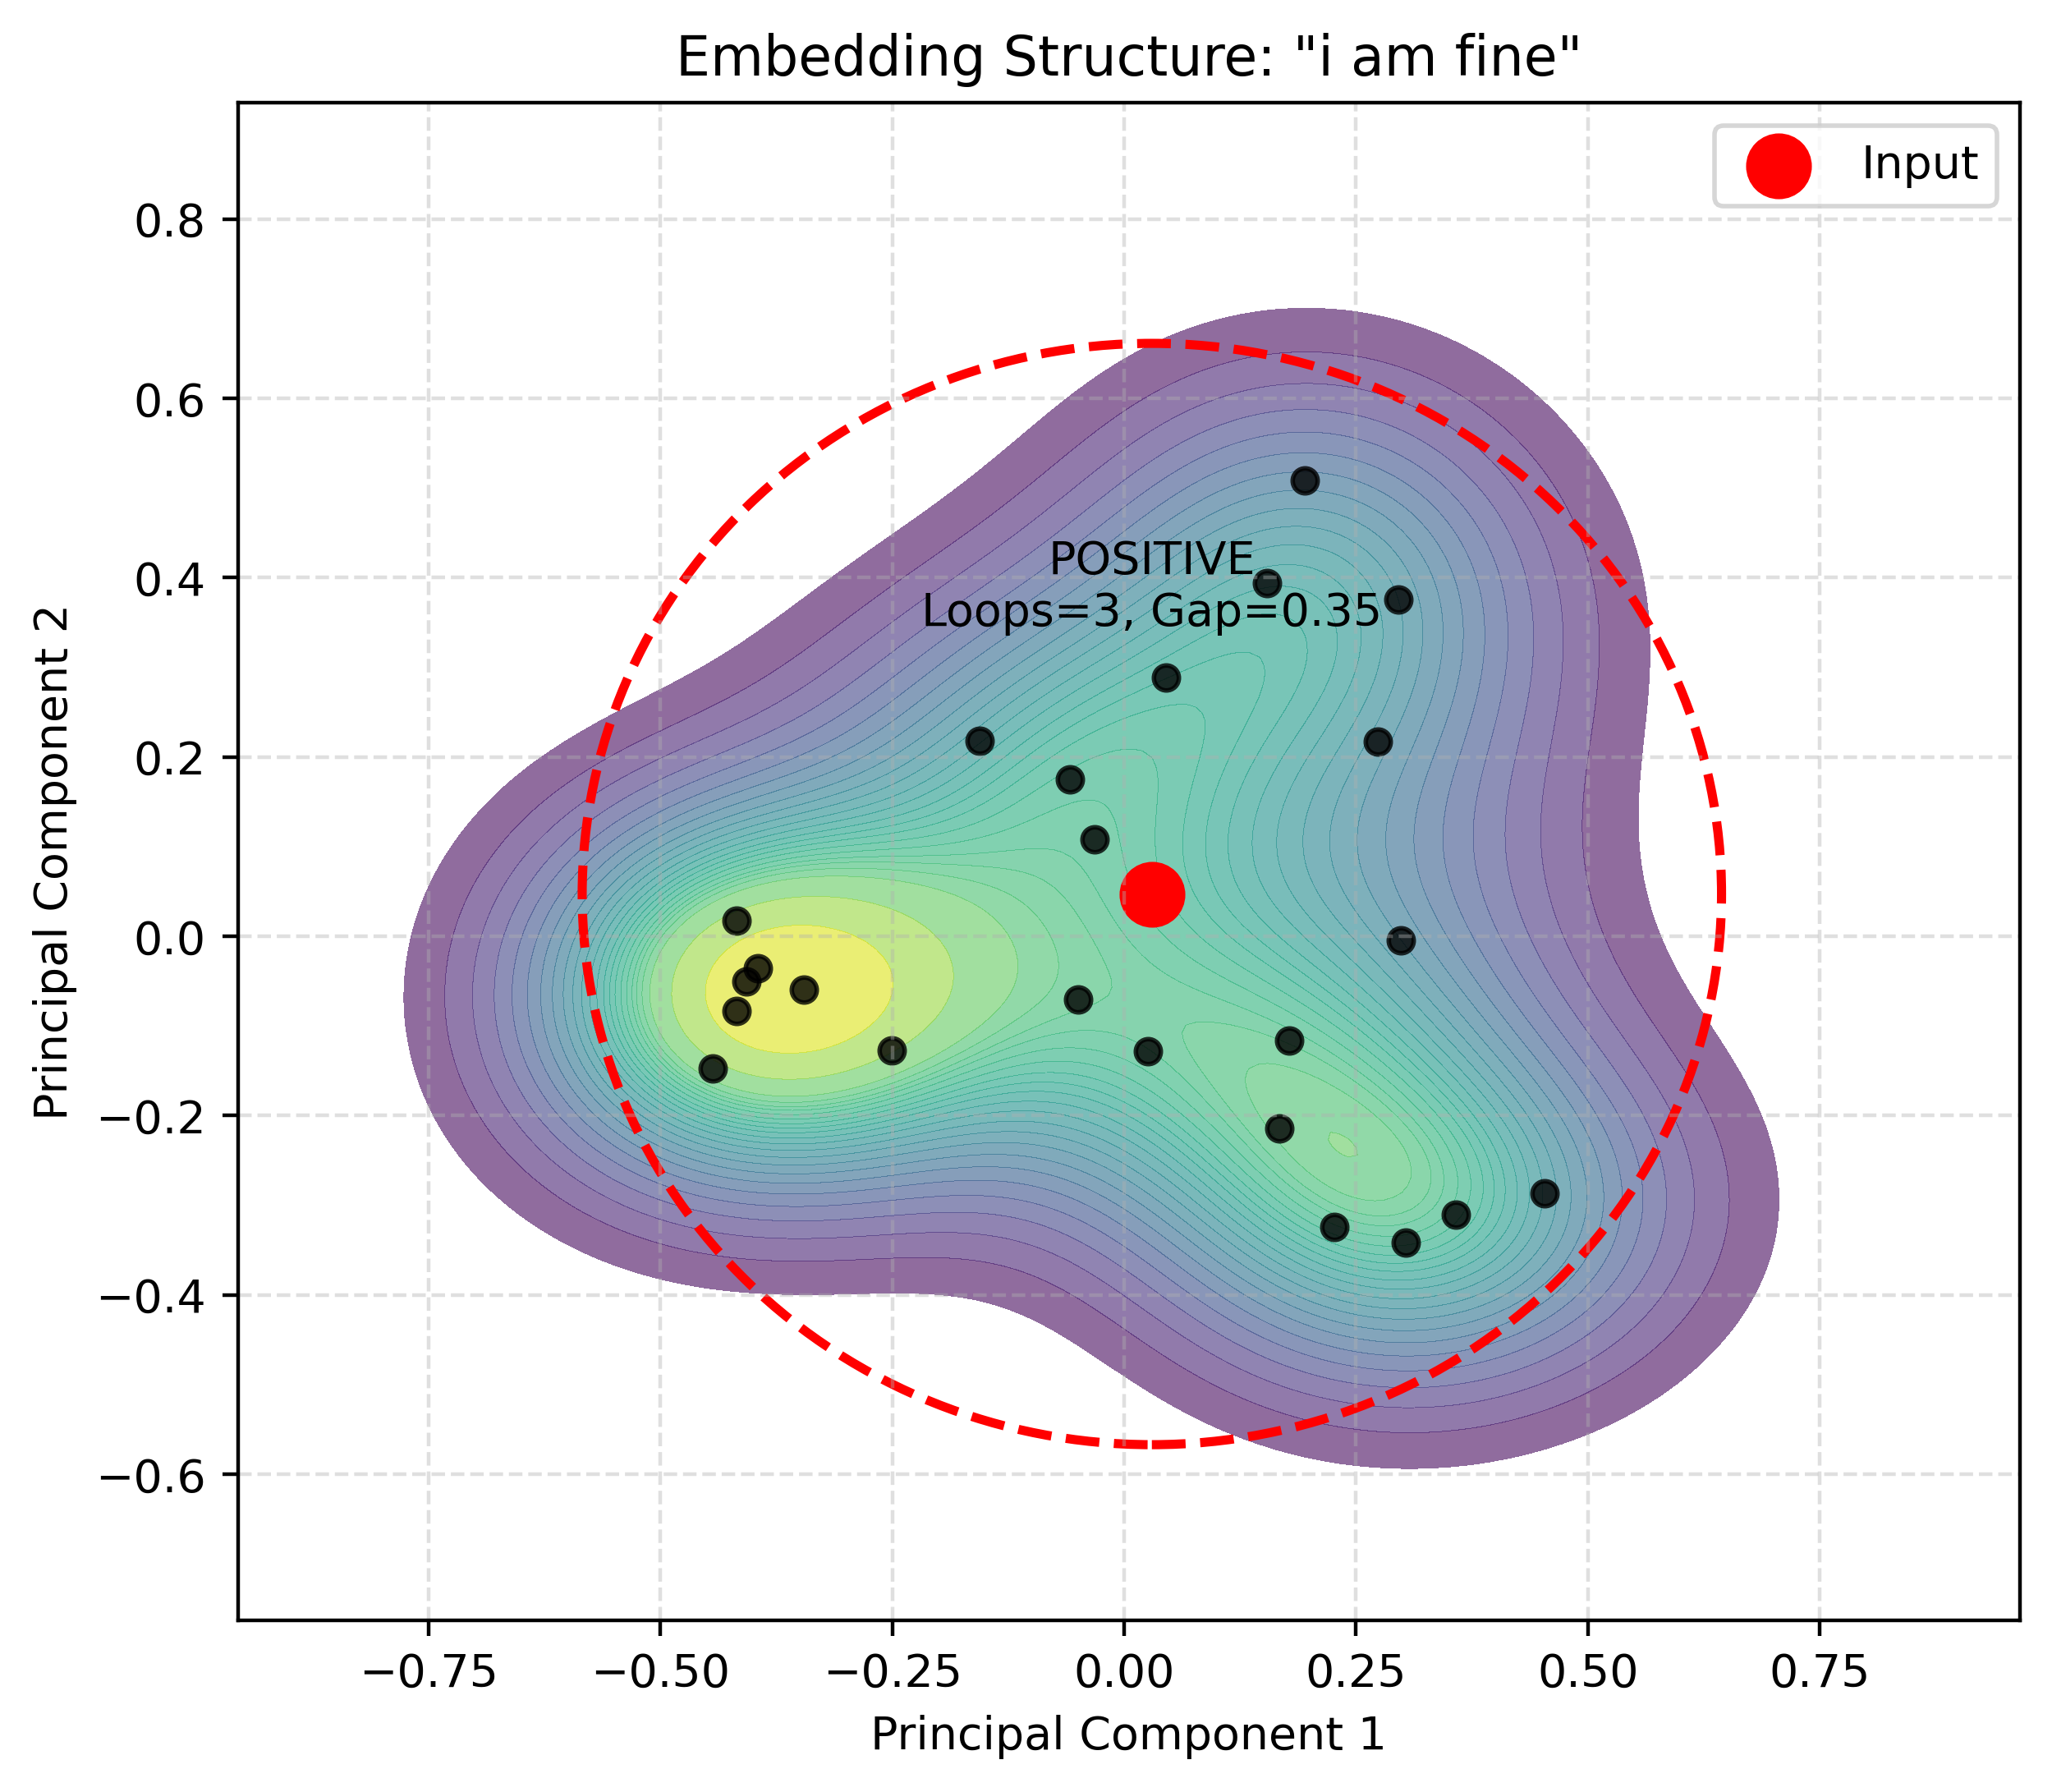
\includegraphics[width=0.85\textwidth]{case1_clear.png}
\caption{Visualization for Case Study 1: ``I Am Fine'' — Clear Topology}
\label{fig:case1}
\end{figure}

As shown in \textbf{Figure~\ref{fig:case1}}, the point cloud for ``I am fine'' forms a
tightly clustered neighbourhood dominated by a single class. The persistence diagram shows
very few H1 features, confirming clean topology and explaining why no ambiguity rule triggers.

\subsection{Case Study 2: I Do Not Know How I Feel}

This case study examines why ``i dont know how i feel'' correctly returns \textsc{ambiguous}.

The debug output for this input is:

\begin{verbatim}
--- DEBUG INFO ---
Input : i dont know how i am feel
Probabilities : POS=0.0991 NEG=0.5271 NEU=0.3794
Confidence gap : 0.1477 (threshold < 0.30)
Loop count (H1): 15 (extreme >= 14, moderate >= 10)
Trigger : EXTREME topology
Final Result : AMBIGUOUS
\end{verbatim}

The loop count of 15 exceeds the extreme threshold of 14, so the first ambiguity rule fires
immediately. The system does not even need to check the confidence gap.

Geometrically, this sentence sits in a complicated region of the embedding space where its 24
nearest neighbours come from very different emotion clusters. The persistence diagram has many
long-lived H1 loops, reflecting this tangled structure. This makes sense: a sentence that
explicitly says ``I do not know how I feel'' should sit near the boundary between multiple
emotion classes, and the topology correctly captures this.

This is exactly the kind of case the system was designed to handle. The sentence is inherently
ambiguous, and the topological analysis detects this in a principled way.

\begin{figure}[H]
\centering
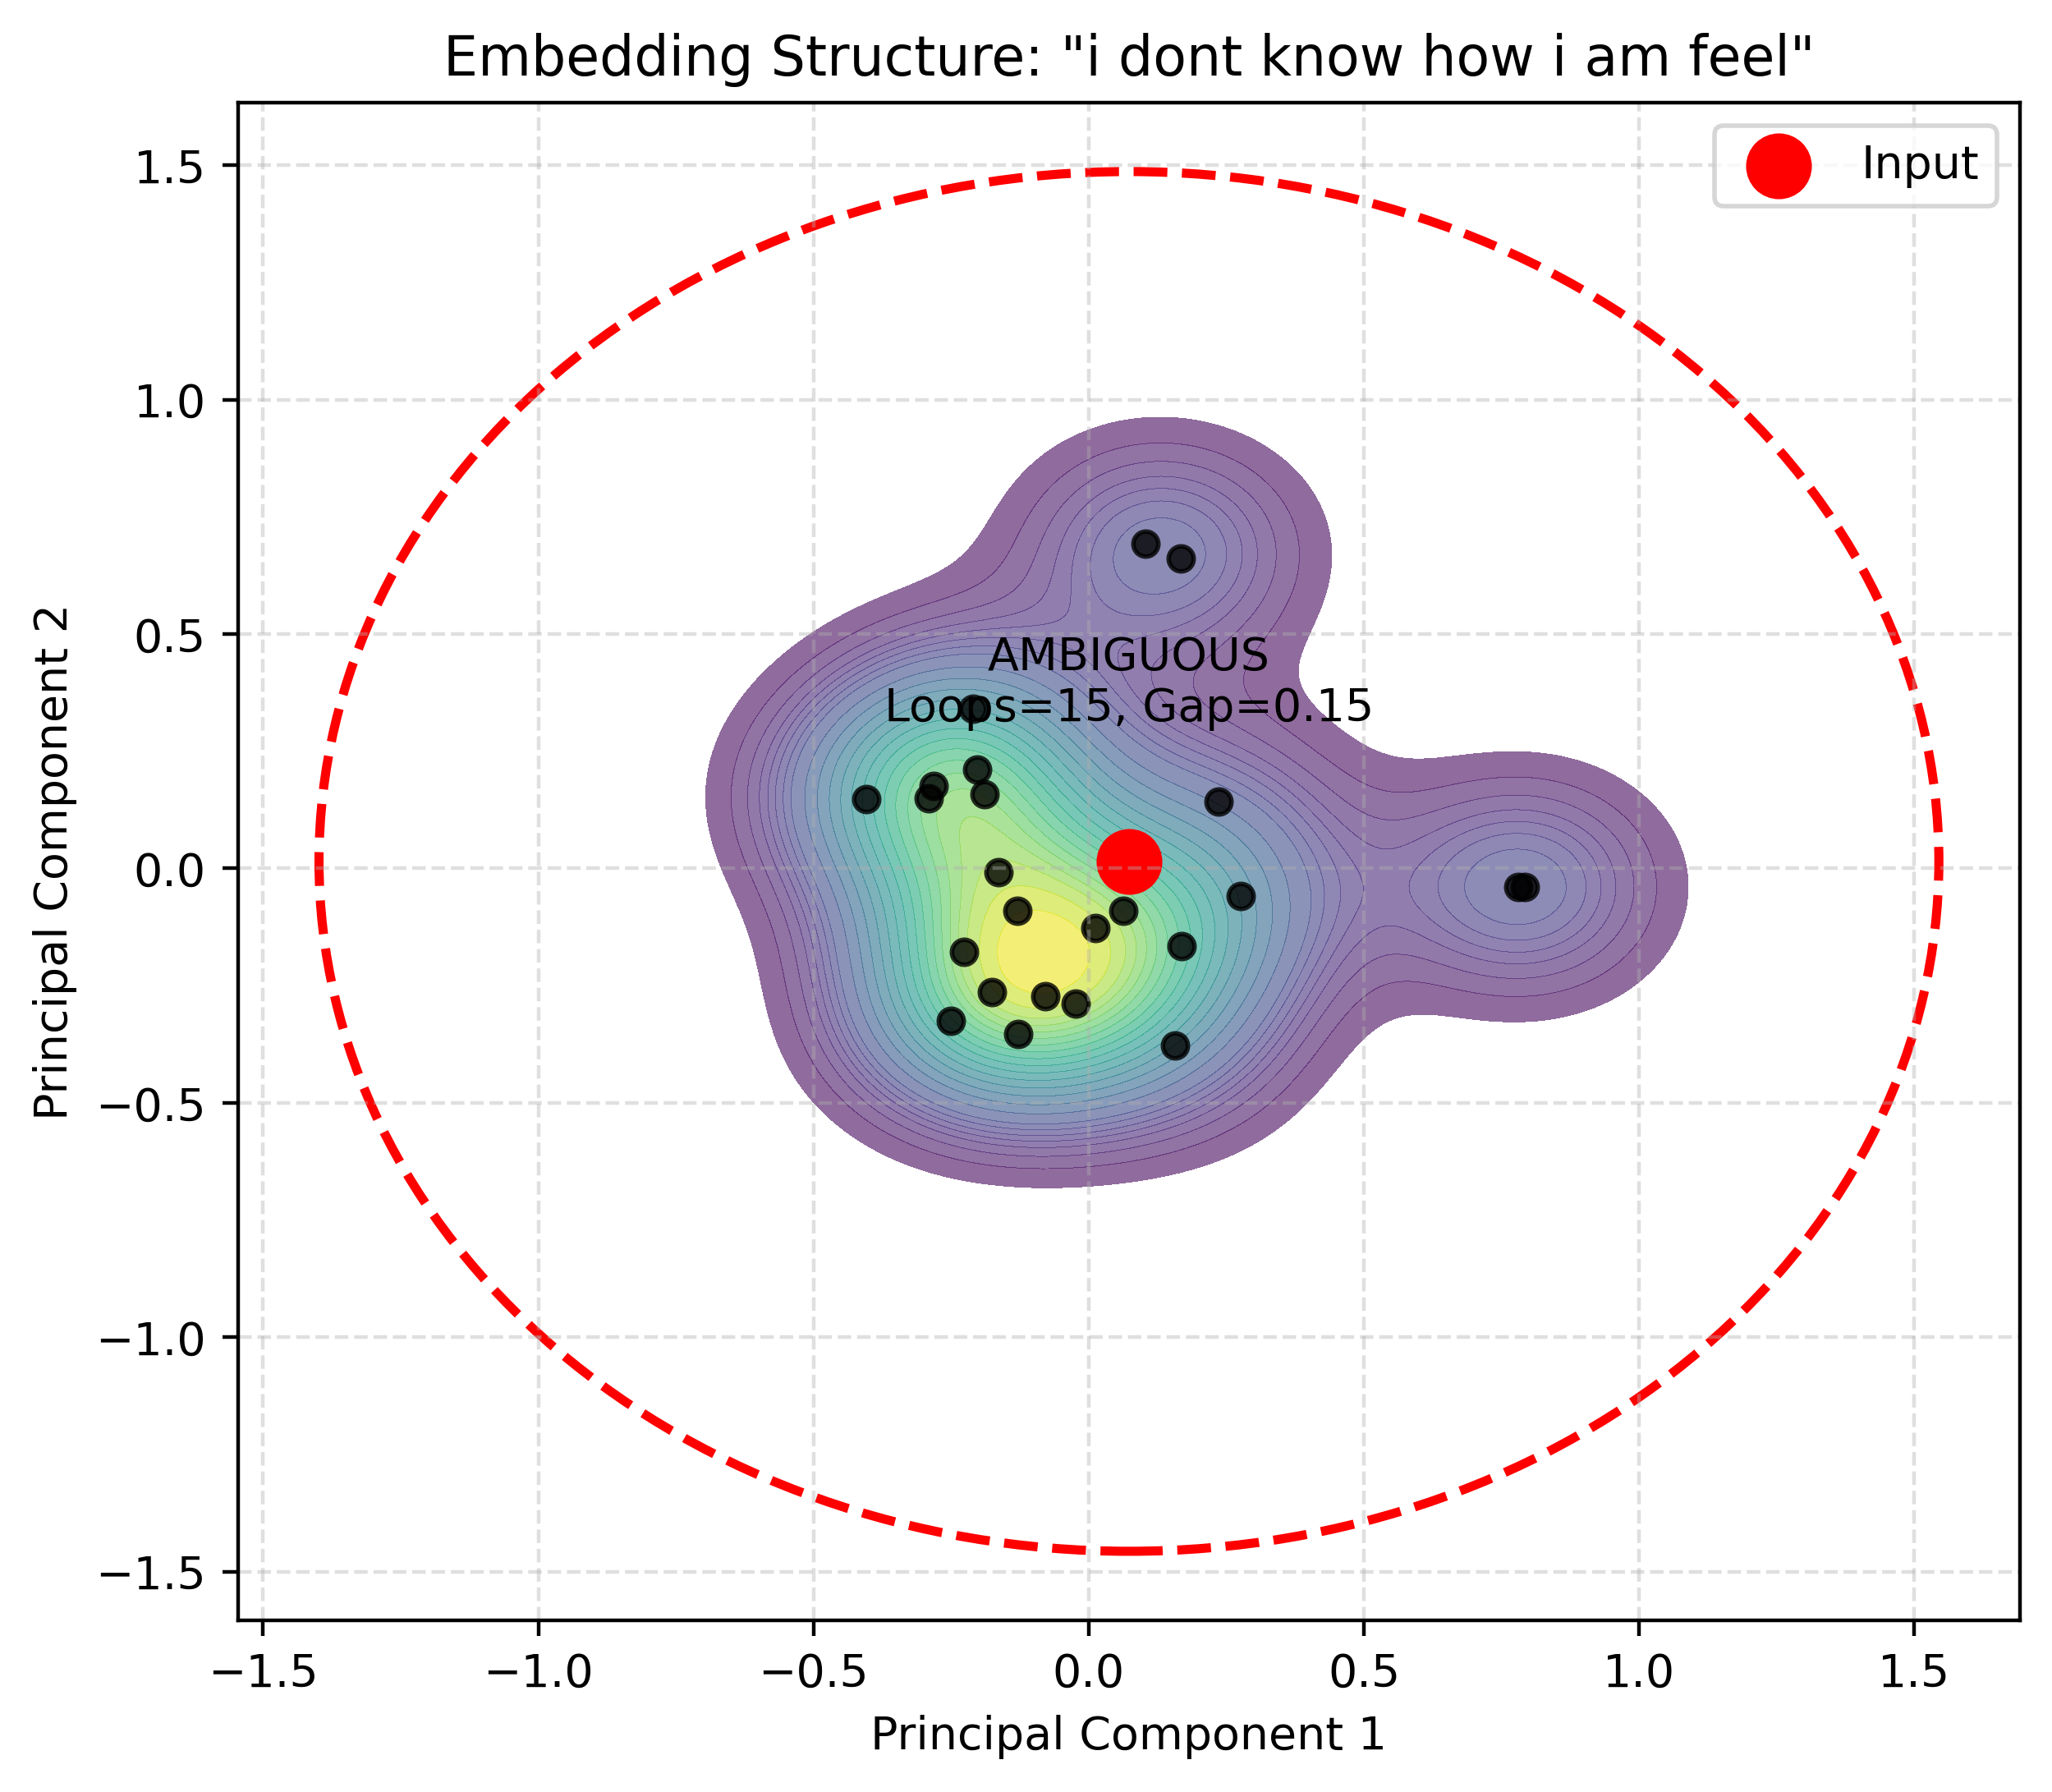
\includegraphics[width=0.85\textwidth]{case2_ambiguous.png}
\caption{Visualization for Case Study 2: ``I Dont Know How I Feel'' — Complex Topology}
\label{fig:case2}
\end{figure}

As shown in \textbf{Figure~\ref{fig:case2}}, the point cloud for this input is scattered
across multiple emotion classes. The persistence diagram reveals numerous long-lived H1 loops,
confirming the geometric complexity that triggers the extreme topology rule.

\section{Timeline of Project Development}

The project was developed over a period of approximately three months. \textbf{Table~\ref{tab:timeline}}
summarizes the major milestones.

\begin{table}[H]
\centering
\caption{Project Development Timeline}
\label{tab:timeline}
\begin{tabular}{lp{9cm}}
\toprule
\textbf{Month} & \textbf{Activities} \\
\midrule
Month 1 (February) &
Literature review. Studied GoEmotions papers and identified the problem of missing ambiguity
detection in existing models. Set up development environment and designed the label mapping. \\
\addlinespace
Month 2 (March) &
Implemented initial version with embeddings and XGBoost. Added TF-IDF features. Integrated
\texttt{giotto-tda} for topology computation. Implemented the ambiguity detection rules. \\
\addlinespace
Month 3 (April) &
Full training on 43,410 samples. Evaluated on test set. Tuned ambiguity thresholds.
Added visualization scripts. Resolved GPU/CPU compatibility issues. Wrote report. \\
\bottomrule
\end{tabular}
\end{table}

As detailed in \textbf{Table~\ref{tab:timeline}}, the project progressed steadily from the initial
literature review phase through to full pipeline implementation, threshold tuning, and formal
evaluation over the span of three months.

\section{Topology Analysis}

During development, the persistence diagrams and point clouds were visualized for several
inputs. The following patterns were observed.

For clearly emotional sentences like ``I am so happy today'', the 24 nearest neighbours in the
embedding space form a tight, well-connected cluster. Almost all neighbours belong to the same
class. The persistence diagram shows very few long-lived H1 features. The confidence gap is
large.

For genuinely ambiguous sentences, the neighbours come from multiple different classes. The
point cloud is scattered. The persistence diagram shows many long-lived H1 features, reflecting
the tangled structure of the neighbourhood. The confidence gap is small.

This confirms that the topological signal is capturing real semantic ambiguity, not just random
noise.

\section{Threshold Sensitivity}

\textbf{Table~\ref{tab:thresh}} shows how the ambiguity rate changes as the loop thresholds are varied
on the test examples.

\begin{table}[H]
\centering
\caption{Effect of Loop Threshold on Ambiguity Rate}
\label{tab:thresh}
\begin{tabular}{ccc}
\toprule
\textbf{Loop Extreme} & \textbf{Loop Moderate} & \textbf{Ambiguity Rate} \\
\midrule
10 & 7  & Higher (around 38\%) \\
14 & 10 & Moderate (around 21\%) \\
18 & 13 & Lower (around 12\%) \\
\bottomrule
\end{tabular}
\end{table}

As indicated in \textbf{Table~\ref{tab:thresh}}, the current thresholds of 14 and 10 were chosen because
they give a meaningful ambiguity rate while not being so aggressive that most inputs are flagged.
Applications that require very confident outputs could raise these thresholds. Applications that
need to flag any uncertain input could lower them.

\section{Performance}

Training takes approximately 3 to 4 hours on CPU for the full 43,410-sample dataset. The
bottleneck is the topology computation step, which runs for every training sample. With
GPU-accelerated embedding encoding, the embedding step is reduced from about 10 minutes to
about 2 minutes, but the topology computation is CPU-bound.

Inference takes approximately 2 to 4 seconds per query on a standard laptop CPU. This is
acceptable for interactive use. The topology computation (finding neighbours and computing
persistence) is the bottleneck at inference time as well.

\section{Limitations}

The known limitations of the current system are:

\begin{itemize}
    \item \textbf{Social Ambiguity Blind Spots:} The system cannot detect social ambiguity
    that is not geometrically visible in the embedding space. ``I am fine'' is a well-known
    socially ambiguous phrase, but it does not appear ambiguous in the geometric sense
    because training data biases its neighbourhood toward clearly Positive samples.

    \item \textbf{Slang and Informal Language:} The system struggles with slang,
    abbreviations, and informal language that is not well-represented in the training data.
    Words like ``yolo'', ``fomo'', ``lol'', and ``idk'' carry emotional meaning but the
    embedding model may not place them accurately because such terms are underrepresented
    in the model's training data. As a result, unusual or newly emerging slang expressions
    may lead to incorrect or ambiguous predictions. This highlights a limitation of
    data-driven models: understanding of language is restricted to patterns seen during
    training. Handling such language would require additional preprocessing using slang
    dictionaries or domain-specific training data.

    \item \textbf{Threshold Calibration:} The ambiguity thresholds were set manually based
    on observation and experimentation. There is no labelled dataset of ``ambiguous social
    media posts'' that could be used for proper threshold calibration.

    \item \textbf{Language Constraint:} The system works only on English text. It was
    trained on Reddit comments and may not generalize well to other social media platforms
    with different writing styles.

    \item \textbf{Inference Bottleneck:} Inference is slower than a standard classifier because
    of the live topology computation. For large-scale deployment, this would need to be
    optimized.
\end{itemize}
